\chapter{Experimentos y Resultados}

En esta sección se describirán los experimentos llevados a cabo y sus resultados. Todas las comparaciones se llevan a cabo mediante una prueba de T de Student desapareada.


\section{Experimento 1} %%%%%%%%%%%%%%%%%%%%%%%%%%%%%%%%%%%%%%%%%%%%%%%%%%%%%%%%%%%%%%%%

El primer paso es hacer una comparación entre los clasificadores individuales y los \ac{ECDD}. El objetivo de este experimento es verificar si efectivamente el desempeño mejora individualmente por cada clasificador, sin hacer una comparación transversal entre clasificadores de distintas familias.

En este experimento también se usó un algoritmo de aprendizaje profundo: \ac{DBN}.

Los resultados del experimento 1 se pueden ver en las Tablas \ref{tab:apurata-proc1}, \ref{tab:lc-proc1} y \ref{tab:german-proc1}.


\subsection{Conjunto de datos Apurata}

El modelo ECDD-LR \textit{(M=$72.56$, SD=$3.48$)} comparado al modelo \ac{LR} \textit{(M=$70.02$, SD=$3.55$)} demostró un \ac{AUC} significativamente mejor, $t(198)=5.11, p=.0001$.

El modelo ECDD-MLP \textit{(M=$70.61$, SD=$3.49$)} comparado al modelo \ac{MLP} \textit{(M=$68.13$, SD=$3.58$)} demostró un \ac{AUC} significativamente mejor, $t(198)=4.96, p=.0001$.

El modelo ECDD-AD \textit{(M=$68.81$, SD=$3.46$)} comparado al modelo \ac{AD} \textit{(M=$61.75$, SD=$6.34$)} demostró un \ac{AUC} significativamente mejor, $t(198)=9.77, p=.0001$.

El modelo ECDD-SVM \textit{(M=$71.70$, SD=$3.54$)} comparado al modelo \ac{SVM} \textit{(M=$66.56$, SD=$3.61$)} demostró un \ac{AUC} significativamente mejor, $t(198)=10.17, p=.0001$.

En resumen, el método propuesto de \textit{bagging} mejoró a los 4 modelos base utilizados.

\begin{table}[htbp]
\centering
\caption{Experimento 1 con conjunto de datos de Apurata}
\label{tab:apurata-proc1}
\begin{tabularx}{0.75\textwidth}{|l|Y Y Y Y|}
				\hline
				& AUC		& Precisión	& Exhaust.		& Exactitud	\\
				\hline
LR				& 70.02		& 89.25		& 96.35			& 82.78		\\		% AUC std: 3.55
ECDD-LR			& 72.56		& 89.76		& 95.96			& 82.86		\\		% AUC std: 3.48
				\hline
MLP				& 68.13		& 88.96		& 91.86			& 80.30		\\		% AUC std: 3.58
ECDD-MLP		& 70.61		& 89.64		& 92.30			& 80.61		\\		% AUC std: 3.49
				\hline
AD				& 61.75		& 86.84		& 98.06			& 83.71		\\		% AUC std: 6.34
ECDD-AD			& 68.81		& 89.42		& 92.93			& 80.73		\\		% AUC std: 3.46
				\hline
SVM				& 66.56		& 89.33		& 87.65			& 78.39		\\		% AUC std: 3.61
ECDD-SVM		& 71.70		& 89.81		& 94.44			& 82.04		\\		% AUC std: 3.54
				\hline
DBN				& 67.80		& 88.04		& 91.76			& 79.84		\\		% AUC std: 3.57
				\hline
\end{tabularx}
\end{table}


\subsection{Conjunto de datos \textit{Lending Club}}

El modelo ECDD-LR \textit{(M=$73.34$, SD=$0.11$)} comparado al modelo \ac{LR} \textit{(M=$73.36$, SD=$0.21$)} demostró una diferencia en \ac{AUC} que no es estadísticamente significativa, $t(198)=0.84, p=.3999$.

El modelo ECDD-MLP \textit{(M=$75.67$, SD=$0.14$)} comparado al modelo \ac{MLP} \textit{(M=$74.87$, SD=$0.18$)} demostró un \ac{AUC} significativamente mejor, $t(198)=35.08, p=.0001$.

El modelo ECDD-AD \textit{(M=$80.34$, SD=$0.12$)} comparado al modelo \ac{AD} \textit{(M=$75.52$, SD=$0.56$)} demostró un \ac{AUC} significativamente mejor, $t(198)=8.16, p=.0001$.

El modelo ECDD-SVM \textit{(M=$74.41$, SD=$0.13$)} comparado al modelo \ac{SVM} \textit{(M=$73.53$, SD=$0.19$)} demostró un \ac{AUC} significativamente mejor, $t(198)=38.22, p=.0001$.

En resumen, el método propuesto de ensamble mejoró a tres de los cuatro modelos base utilizados. Es interesante notar que el modelo base \ac{LR} que no mejoró con la propuesta, es también aquel que tiene el \ac{AUC} promedio más bajo del conjunto.

\begin{table}[htbp]
\centering
\caption{Experimento 1 con conjunto de datos de \textit{Lending Club}}
\label{tab:lc-proc1}
\begin{tabularx}{0.75\textwidth}{|l|Y Y Y Y|}
				\hline
				& AUC		& Precisión	& Exhaust.		& Exactitud	\\
				\hline
LR				& 73.36		& 77.83		& 95.40			& 75.05		\\		% AUC std: 0.21
ECDD-LR			& 73.34		& 77.55		& 96.23			& 74.85		\\		% AUC std: 0.11
				\hline
MLP				& 74.87		& 78.29		& 95.74			& 75.71		\\		% AUC std: 0.18
ECDD-MLP		& 75.67		& 79.09		& 94.07			& 75.82		\\		% AUC std: 0.14
				\hline
AD				& 75.52		& 77.94		& 92.86			& 75.34		\\		% AUC std: 0.56
ECDD-AD			& 80.34		& 81.88		& 89.50			& 78.05		\\		% AUC std: 0.12
				\hline
SVM				& 73.53		& 77.42		& 97.29			& 75.03		\\		% AUC std: 0.19
ECDD-SVM		& 74.41		& 78.29		& 95.91			& 75.00		\\		% AUC std: 0.13
				\hline
DBN				& 75.01		& 78.56		& 94.92			& 75.72		\\		% AUC std: 0.23
				\hline
\end{tabularx}
\end{table}


\subsection{Conjunto de datos Alemán}

El modelo ECDD-LR \textit{(M=$71.50$, SD=$2.02$)} comparado al modelo \ac{LR} \textit{(M=$71.45$, SD=$3.12$)} demostró una diferencia en \ac{AUC} que no es estadísticamente significativa, $t(198)=0.13, p=.8931$.

El modelo ECDD-MLP \textit{(M=$71.61$, SD=$2.10$)} comparado al modelo \ac{MLP} \textit{(M=$69.36$, SD=$3.63$)} demostró un \ac{AUC} significativamente mejor, $t(198)=26.83, p=.0001$.

El modelo ECDD-AD \textit{(M=$71.82$, SD=$1.99$)} comparado al modelo \ac{AD} \textit{(M=$66.86$, SD=$5.52$)} demostró un \ac{AUC} significativamente mejor, $t(198)=8.45, p=.0001$.

El modelo ECDD-SVM \textit{(M=$71.49$, SD=$2.09$)} comparado al modelo \ac{SVM} \textit{(M=$67.54$, SD=$3.34$)} demostró un \ac{AUC} significativamente mejor, $t(198)=10.03, p=.0001$.

En resumen, el método propuesto de ensamble mejoró a tres de los cuatro modelos base utilizados. Es interesante notar que el modelo base \ac{LR} que no mejoró con la propuesta, es también aquel que tiene el \ac{AUC} promedio más alto del conjunto.


\begin{table}[htbp]
\centering
\caption{Experimento 1 con conjunto de datos Alemán}
\label{tab:german-proc1}
\begin{tabularx}{0.75\textwidth}{|l|Y Y Y Y|}
				\hline
				& AUC		& Precisión	& Exhaust.		& Exactitud	\\
				\hline
LR				& 71.45		& 81.77		& 99.32			& 78.92		\\		% AUC std: 3.12
ECDD-LR			& 71.50		& 81.84		& 98.83			& 78.68		\\		% AUC std: 2.02
				\hline
MLP				& 69.36		& 81.26		& 98.76			& 78.78		\\		% AUC std: 3.63
ECDD-MLP		& 71.61		& 82.44		& 97.08			& 79.00		\\		% AUC std: 2.10
				\hline
AD				& 66.86		& 79.48		& 99.85			& 78.35		\\		% AUC std: 5.52
ECDD-AD			& 71.82		& 82.71		& 96.02			& 79.20		\\		% AUC std: 1.99
				\hline
SVM				& 67.54		& 80.79		& 97.28			& 79.12		\\		% AUC std: 3.34
ECDD-SVM		& 71.49		& 82.27		& 97.88			& 79.35		\\		% AUC std: 2.09
				\hline
DBN				& 66.84		& 80.07		& 97.98			& 78.24		\\		% AUC std: 3.68
				\hline
\end{tabularx}
\end{table}

\subsection{Sobre el aprendizaje profundo}

El caso de la \ac{DBN} es particular. En primer lugar, ajustar los parámetros del modelo resulta complejo, porque tiene numerosos parámetros y porque al ser pocos datos el modelo presenta una tendencia al \textit{overfitting}. Esto se observa al tener un desempeño impecable con los datos de entrenamiento, pero un desempeño muy inferior con los datos de prueba.

En el conjunto de datos Apurata, el modelo DBN \textit{(M=$67.80$, SD=$3.57$)} comparado al modelo \ac{LR} \textit{(M=$70.02$, SD=$3.55$)} demostró un \ac{AUC} significativamente peor, $t(198)=4.41, p=.0001$.

En el conjunto de datos Apurata, el modelo DBN \textit{(M=$67.80$, SD=$3.57$)} comparado al modelo ECDD-LR \textit{(M=$72.56$, SD=$3.48$)} demostró un \ac{AUC} significativamente peor, $t(198)=9.55, p=.0001$.

En el conjunto de datos \textit{Lending Club}, el modelo DBN \textit{(M=$75.01$, SD=$0.23$)} comparado al modelo \ac{AD} \textit{(M=$75.52$, SD=$0.56$)} demostró un \ac{AUC} significativamente peor, $t(198)=8.42, p=.0001$.

En el conjunto de datos \textit{Lending Club}, el modelo DBN \textit{(M=$75.01$, SD=$0.23$)} comparado al modelo ECDD-AD \textit{(M=$80.34$, SD=$0.12$)} demostró un \ac{AUC} significativamente peor, $t(198)=205.46, p=.0001$.

En el conjunto de datos Alemán, el modelo DBN \textit{(M=$66.84$, SD=$3.68$)} comparado al modelo \ac{LR} \textit{(M=$71.45$, SD=$3.12$)} demostró un \ac{AUC} significativamente peor, $t(198)=9.56, p=.0001$.

En el conjunto de datos Alemán, el modelo DBN \textit{(M=$66.84$, SD=$3.68$)} comparado al modelo ECDD-AD \textit{(M=$71.82$, SD=$1.99$)} demostró un \ac{AUC} significativamente peor, $t(198)=11.90, p=.0001$.

Luego de ajustar cuidadosamente los parámetros de la mejor forma posible, el \ac{AUC} es peor que otros clasificadores base. Esto se puede explicar con la baja dimensionalidad de los datos y la poca cantidad de instancias; ya que no se explota la capacidad de reducción de dimensionalidad del modelo y tampoco se hace un entrenamiento adecuado por la escasez de datos.

En conclusión, este clasificador no es adecuado para este problema, y al ser bastante complejo en sí mismo, no se le creó una versión ensamblada.


\subsection{Conclusiones del Experimento 1}

Debido a la densidad de los resultados, se creó la Tabla \ref{tab:summary1_2} con un resumen cualitativo de los experimentos 1 y 2. De forma que se facilite la lectura de las conclusiones.

Se vio que aplicando la propuesta de ensamble, el \ac{AUC} mejoró en prácticamente todos los clasificadores base, excepto las \ac{LR} en dos conjuntos de datos.

La exhaustividad promedio disminuye en la mayoría de modelos, ya que existe un balance entre la precisión y la exhaustividad. Y ya que se trató de optimizar la exactitud, indirectamente se optimizó la precisión, de forma que la exhaustividad disminuyó.

Se ve claramente que el árbol de decisión fue el algoritmo base que mejora más su \ac{AUC} promedio con el método \ac{ECDD}. Esto se debe a que individualmente el árbol de decisión es muy sensible al ruido y fácilmente hace \textit{overfitting}. Sin embargo al ponerlo dentro de un ensamble, su capacidad de generalizar mejora. De hecho es la misma razón por la que los algoritmos de ensamble del estado del arte actualmente usan árboles de decisión como su clasificador base.




\section{Experimento 2} %%%%%%%%%%%%%%%%%%%%%%%%%%%%%%%%%%%%%%%%%%%%%%%%%%%%%%%%%%%%%%%%

En este experimento se comparará los \ac{ECDD} con dos algoritmos de \textit{bagging} usados ampliamente en la actualidad: \ac{RF} y \ac{XGBoost}. El objectivo de este experimento es verificar que el método de \ac{ECDD} es competitivo con otros métodos de ensamble del estado del arte, sin el sesgo de haber usado una metodología diferente para el entrenamiento y la evaluación de los modelos.

Los resultados del experimento 2 se pueden ver en las Tablas \ref{tab:apurata-proc2}, \ref{tab:lc-proc2} y \ref{tab:german-proc2}.

\subsection{Conjunto de datos Apurata}

De entre los modelos propuestos, el que tiene un \ac{AUC} promedio más elevado es ECDD-LR, y el que tiene un \ac{AUC} promedio más bajo es ECDD-AD. A continuación se compararán ambos modelos con \ac{RF} y \ac{XGBoost}.

El modelo ECDD-LR \textit{(M=$72.56$, SD=$3.48$)} comparado al modelo \ac{RF} \textit{(M=$69.23$, SD=$3.52$)} demostró un \ac{AUC} significativamente mejor, $t(198)=6.73, p=.0001$.

El modelo ECDD-AD  \textit{(M=$68.81$, SD=$3.46$)} comparado al modelo \ac{RF} \textit{(M=$69.23$, SD=$3.52$)} demostró una diferencia en \ac{AUC} que no es estadísticamente significativa, $t(198)=0.85, p=.3958$.

El modelo ECDD-LR \textit{(M=$72.56$, SD=$3.48$)} comparado al modelo \ac{XGBoost} \textit{(M=$67.91$, SD=$3.47$)} demostró un \ac{AUC} significativamente mejor, $t(198)=9.46, p=.0001$.

El modelo ECDD-AD \textit{(M=$68.81$, SD=$3.46$)} comparado al modelo \ac{XGBoost} \textit{(M=$67.91$, SD=$3.47$)} demostró una diferencia en \ac{AUC} que no es estadísticamente significativa, $t(198)=1.84, p=.0678$.

En resumen, los modelos propuestos son competitivos e incluso superan a los modelos del estado del arte en este conjunto de datos particular.

\begin{table}[htbp]
\centering
\caption{Experimento 2 con conjunto de datos de Apurata}
\label{tab:apurata-proc2}
\begin{tabularx}{0.75\textwidth}{|l|Y Y Y Y|}
				\hline
				& AUC		& Precisión	& Exhaust.		& Exactitud	\\
				\hline
ECDD-LR			& 72.56		& 89.76		& 95.96			& 82.86		\\		% AUC std: 3.48
ECDD-MLP	 	& 70.61		& 89.64		& 92.30			& 80.61		\\		% AUC std: 3.49
ECDD-AD			& 68.81		& 89.42		& 92.93			& 80.73		\\		% AUC std: 3.46
ECDD-SVM	 	& 71.70		& 89.81		& 94.44			& 82.04		\\		% AUC std: 3.54
				\hline
RF		 		& 69.23		& 89.37		& 94.57			& 81.66		\\		% AUC std: 3.52
XGB				& 67.91		& 89.31		& 89.92			& 78.75		\\		% AUC std: 3.47
				\hline
\end{tabularx}
\end{table}

\subsection{Conjunto de datos de \textit{Lending Club}}

De entre los modelos propuestos, el que tiene un \ac{AUC} promedio más elevado es ECDD-AD, y el que tiene un \ac{AUC} promedio más bajo es ECDD-SVM. A continuación se compararán ambos modelos con \ac{RF} y \ac{XGBoost}.

El modelo ECDD-AD \textit{(M=$71.82$, SD=$0.12$)} comparado al modelo \ac{RF} \textit{(M=$71.32$, SD=$0.14$)} demostró un \ac{AUC} significativamente mejor, $t(198)=27.12, p=.0001$.

El modelo ECDD-SVM  \textit{(M=$71.49$, SD=$0.13$)} comparado al modelo \ac{RF} \textit{(M=$71.32$, SD=$0.14$)} demostró un \ac{AUC} significativamente mejor, $t(198)=8.90, p=.0001$.

El modelo ECDD-AD \textit{(M=$71.82$, SD=$0.12$)} comparado al modelo \ac{XGBoost} \textit{(M=$70.68$, SD=$0.12$)} demostró un \ac{AUC} significativamente mejor, $t(198)=67.18, p=.0001$.

El modelo ECDD-SVM \textit{(M=$71.49$, SD=$0.13$)} comparado al modelo \ac{XGBoost} \textit{(M=$70.68$, SD=$0.12$)} demostró un \ac{AUC} significativamente mejor, $t(198)=45.78, p=.0001$.

En resumen, los modelos propuestos son mejores que los modelos del estado del arte en este conjunto de datos.

\begin{table}[htbp]
\centering
\caption{Experimento 2 con conjunto de datos de \textit{Lending Club}}
\label{tab:lc-proc2}
\begin{tabularx}{0.75\textwidth}{|l|Y Y Y Y|}
				\hline
				& AUC		& Precisión	& Exhaust.		& Exactitud	\\
				\hline
ECDD-LR			& 71.50		& 81.84		& 98.83			& 78.68		\\		% AUC std: 0.12
ECDD-MLP		& 71.61		& 82.44		& 97.08			& 79.00		\\		% AUC std: 0.14
ECDD-AD			& 71.82		& 82.71		& 96.02			& 79.20		\\		% AUC std: 0.12
ECDD-SVM		& 71.49		& 82.27		& 97.88			& 79.35		\\		% AUC std: 0.13
				\hline
RF				& 71.32		& 82.18		& 97.23			& 78.79		\\		% AUC std: 0.14
XGB				& 70.68		& 81.89		& 98.56			& 78.81		\\		% AUC std: 0.12
				\hline
\end{tabularx}
\end{table}

\subsection{Conjunto de datos Alemán}

De entre los modelos propuestos, el que tiene un \ac{AUC} promedio más elevado es ECDD-AD, y el que tiene un \ac{AUC} promedio más bajo es ECDD-LR. A continuación se compararán ambos modelos con \ac{RF} y \ac{XGBoost}.

El modelo ECDD-AD \textit{(M=$80.34$, SD=$2.09$)} comparado al modelo \ac{RF} \textit{(M=$79.82$, SD=$2.14$)} demostró una diferencia en \ac{AUC} que no es estadísticamente significativa, $t(198)=1.74, p=.0837$.

El modelo ECDD-LR  \textit{(M=$73.34$, SD=$2.12$)} comparado al modelo \ac{RF} \textit{(M=$79.82$, SD=$2.14$)} demostró un \ac{AUC} significativamente peor, $t(198)=21.52, p=.0001$.

El modelo ECDD-AD \textit{(M=$80.34$, SD=$2.09$)} comparado al modelo \ac{XGBoost} \textit{(M=$80.28$, SD=$2.08$)} demostró una diferencia en \ac{AUC} que no es estadísticamente significativa, $t(198)=0.20, p=.8390$.

El modelo ECDD-LR \textit{(M=$73.34$, SD=$2.12$)} comparado al modelo \ac{XGBoost} \textit{(M=$80.28$, SD=$2.08$)} demostró un \ac{AUC} significativamente peor, $t(198)=23.37, p=.0001$.

En resumen, los modelos propuestos son competitivos pero no alcanzan a superar a los modelos del estado del arte en este conjunto de datos.

\begin{table}[htbp]
\centering
\caption{Experimento 2 con conjunto de datos Alemán}
\label{tab:german-proc2}
\begin{tabularx}{0.75\textwidth}{|l|Y Y Y Y|}
				\hline
				& AUC		& Precisión	& Exhaust.		& Exactitud	\\
				\hline
ECDD-LR			& 73.34		& 77.55		& 96.23			& 74.85		\\		% AUC std: 2.12
ECDD-MLP		& 75.67		& 79.09		& 94.07			& 75.82		\\		% AUC std: 2.10
ECDD-AD			& 80.34		& 81.88		& 89.50			& 78.05		\\		% AUC std: 2.09
ECDD-SVM		& 74.41		& 78.29		& 95.91			& 75.00		\\		% AUC std: 2.19
				\hline
RF				& 79.82		& 80.84		& 92.01			& 76.22		\\		% AUC std: 2.14
XGB				& 80.28		& 81.43		& 91.66			& 78.93		\\		% AUC std: 2.08
				\hline
\end{tabularx}
\end{table}

\subsection{Conclusiones del Experimento 2}

Nuevamente se puede consultar la Tabla \ref{tab:summary1_2} para facilitar la lectura de las conclusiones.

Se observó que en los conjuntos de datos de Apurata y \textit{Lending Club}, se consiguió superar el desempeño de \ac{RF} y \ac{XGBoost}. En cambio, en el conjunto de datos Alemán se obtuvo un desempeño similar con los árboles de decisión y peor con \ac{LR}. En consecuencia, se puede afirmar que el método propuesto mejora o al menos mantiene un desempeño similar a modelos del estado del arte. Los resultados varían según el clasificador base utilizado y el conjunto de datos.

Lamentablemente no es posible extrapolar estas conclusiones a otros dominios donde también hayan conjuntos de datos desbalanceados, ya que los conjuntos de datos crediticios además del desbalance poseen otras características que podrían no cumplirse en otros dominios, como la estacionalidad de los datos, la baja cantidad de variables y la información parcialmente oculta. De modo que no se puede afirmar que estos \ac{ECDD} son universalmente mejores que \textit{Random Forest} y \textit{XGBoost}.

Otra observación interesante es el buen desempeño que obtiene la Regresión Logística en el conjunto de Apurata. Esto podría indicar que la información es linealmente separable y los otros modelos sufren de \textit{overfitting}, razón por la cuál su desempeño no es óptimo.

Finalmente, el \ac{ECDD} de árboles de decisión obtiene resultados muy buenos consistentemente en \textit{Lending Club} y el Crédito Alemán, lo que sugiere que si los datos no son linealmente separables, entonces este modelo tiene un gran desempeño. Probando una vez más que usar los árboles de decisión como base para algoritmos de ensamble tiene muy buenos resultados.

\begin{table}[htbp]
    \centering
    \caption{Resumen de los experimentos 1 y 2}
    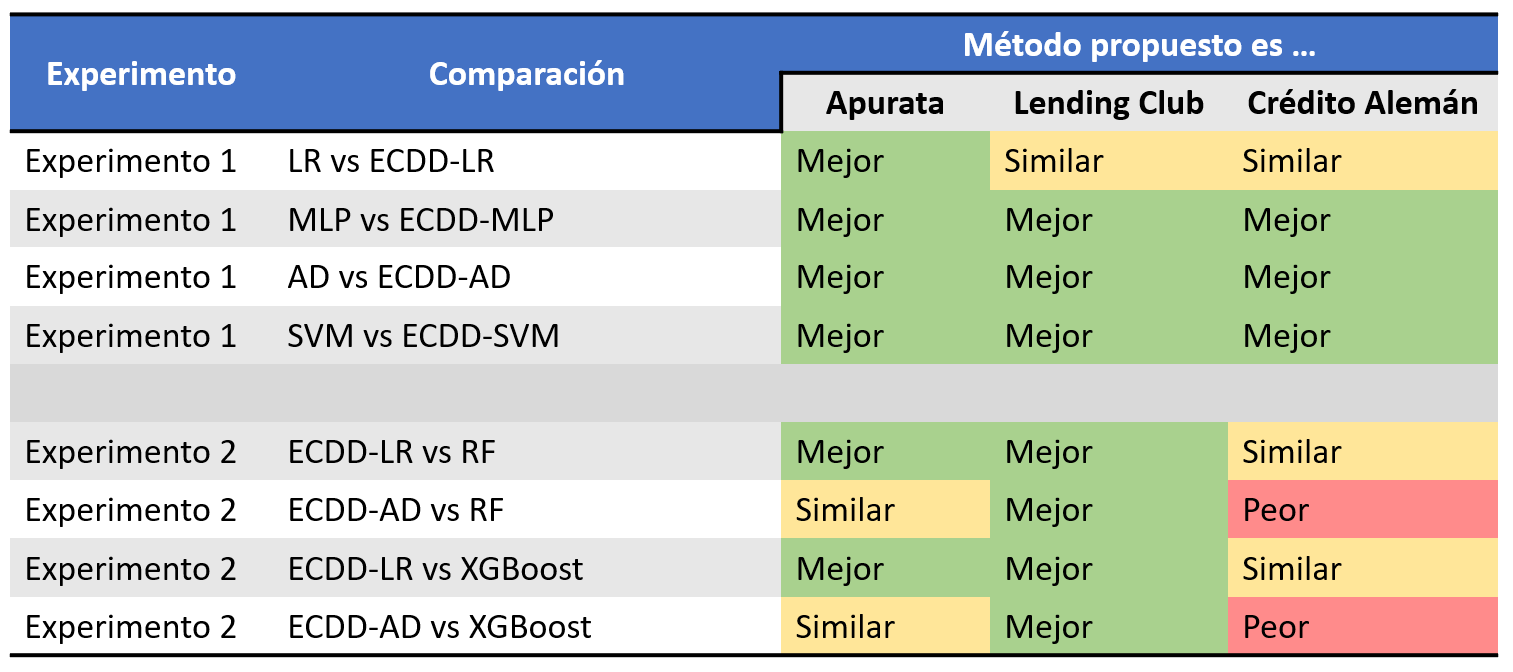
\includegraphics[width=\linewidth]{graficos/propios/resumen_experimentos1_2.PNG}
    \label{tab:summary1_2}
\end{table}

\section{Experimento 3} %%%%%%%%%%%%%%%%%%%%%%%%%%%%%%%%%%%%%%%%%%%%%%%%%%%%%%%%%%%%%%%%

En este experimento se compararon los resultados obtenidos por los modelos \ac{ECDD} con los resultados obtenidos en otros estudios del estado del arte que usan los mismos conjuntos de datos. El objetivo de este experimento es ratificar que los resultados son válidos para el estado del arte usando dos conjuntos de datos referenciales.

Los resultados del experimento 3 se pueden ver en las Tablas \ref{tab:lc-proc3} y \ref{tab:german-proc3}. Sólo se tienen resultados para \textit{Lending Club} y el Cŕedito Alemán puesto que Apurata es un conjunto de datos privado que es usado de forma inédita en esta tesis.

Para una comprensión rápida de los resultados se creó la Tabla \ref{tab:summary3}, de forma análoga a los experimentos anteriores.

\begin{table}[htbp]
\centering
\caption{Experimento 3 con conjunto de datos de \textit{Lending Club}}
\label{tab:lc-proc3}
\begin{tabularx}{\textwidth}{|l|Y Y l|}
				\hline
				& AUC			& Exactitud		& Ref.									\\
				\hline
ECDD-LR			& 71.50			& 78.68			&										\\		% AUC std: 0.12
ECDD-MLP		& 71.61			& 79.00			&										\\		% AUC std: 0.14
ECDD-AD			& 71.82			& 79.20			&										\\		% AUC std: 0.12
ECDD-SVM		& 71.49			& 79.35			&										\\		% AUC std: 0.13
				\hline
RF				& 71.00			& 78.00			& Malekipirbazari, M.et al (2015)		\\		% No std data
SVM				& 62.00			& 63.30			& Malekipirbazari, M.et al (2015)		\\		% No std data
AD				& -				& 81.22			& Zhang, Y. Et al (2016)				\\		% No std data
NN				& -				& 77.40			& Zhang, Y. Et al (2016)				\\		% No std data
MLP				& -				& 78.60			& Zang, D. et al (2015)					\\		% No std data
crDNN			& 72.55			& -				& Tan, F. et al (2018)					\\		% AUC std: 0.32
LR				& 71.52			& -				& Tan, F. et al (2018)					\\		% AUC std: 0.31
mcDNN			& 70.88			& -				& Tan, F. et al (2018)					\\		% AUC std: 0.28
CRSA			& 69.30			& -				& Tan, F. et al (2018)					\\		% AUC std: 0.44
				\hline
\end{tabularx}
\par
\end{table}


\begin{table}[htbp]
\centering
\caption{Experimento 3 con conjunto de datos Alemán}
\label{tab:german-proc3}
\begin{tabularx}{\textwidth}{|l|Y Y l|}
						\hline
						& AUC		& Exactitud	& Ref.									\\
						\hline
ECDD-LR					& 73.34		& 74.85		&										\\		% AUC std: 2.12
ECDD-MLP				& 75.67		& 75.82		&										\\		% AUC std: 2.10
ECDD-AD					& 80.34		& 78.05		&										\\		% AUC std: 2.09
ECDD-SVM				& 74.41		& 75.00		&										\\		% AUC std: 2.19
						\hline
SVM-linear				& 69.13		& 78.70		& Harris, T. (2015)						\\		% AUC std: 2.94
SVM-RBF					& 69.53		& 78.00		& Harris, T. (2015)						\\		% AUC std: 2.92
CSVM-RBF				& 69.23		& 77.10		& Harris, T. (2015)						\\		% AUC std: 3.17
MLP						& 78.09		& 75.20		& Nanni, L. \& Lumini, A. (2009)		\\		% No std data
Rand Subsp LMNC			& 78.47		& 73.93		& Nanni, L. \& Lumini, A. (2009)		\\		% No std data
Bagging MLP				& 79.32		& 75.33		& Nanni, L. \& Lumini, A. (2009)		\\		% No std data
Class Switch MLP		& 78.62		& 73.93		& Nanni, L. \& Lumini, A. (2009)		\\		% No std data
Rotat Forest MLP		& 79.39		& 75.00		& Nanni, L. \& Lumini, A. (2009)		\\		% No std data
Lin LS-SVM				& 81.90		& -			& Brown, I. \& Mues, C. (2012)			\\		% No std data
Random Forests			& 80.00		& -			& Brown, I. \& Mues, C. (2012)			\\		% No std data
RS-Bagging AD			& -			& 78.36		& Wang, G. et al. (2012)				\\		% No std data
Bagging-RS AD			& -			& 78.52		& Wang, G. et al. (2012)				\\		% No std data
						\hline
\end{tabularx}
\par
\end{table}


Los modelos utilizados en los estudios referenciales son bastante diversos, abarcando modelos lineales y no lineales, de árboles y redes neuronales, llegando incluso a incluir redes neuronales profundas.

Es importante notar que al haber seguido procesos diferentes, los resultados de diferentes estudios son más difíciles de comparar. Es por esto que las conclusiones del experimento 2 son tan importantes.

Cinco de los siete estudios referenciales no incluyen la desviación estándar en sus resultados, así que resulta imposible realizar una prueba de significancia estadística. Pero revisando el \ac{AUC} promedio, se puede notar que los resultados son efectivamente competitivos con el estado del arte en calificación crediticia.

\begin{table}[htbp]
    \centering
    \caption{Resumen del experimento 3}
    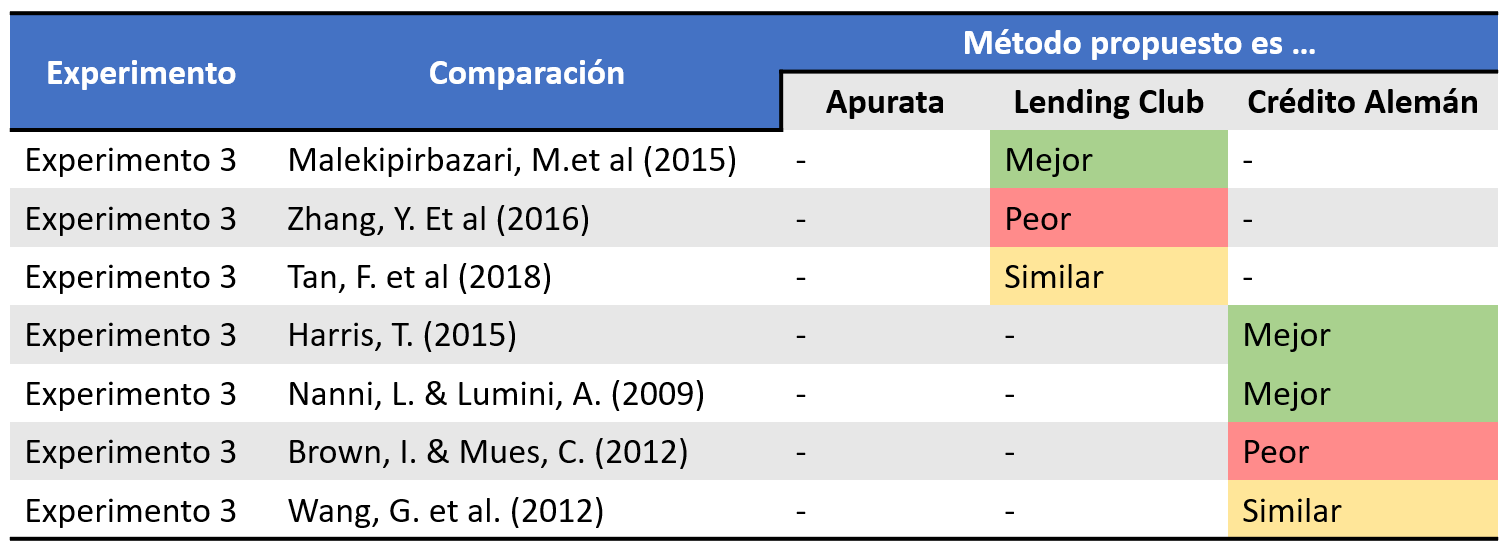
\includegraphics[width=\linewidth]{graficos/propios/resumen_experimento3.PNG}
    \label{tab:summary3}
\end{table}
